\documentclass[border=10pt]{standalone}
\usepackage{tikz}
\usetikzlibrary{automata, positioning, arrows}

\begin{document}
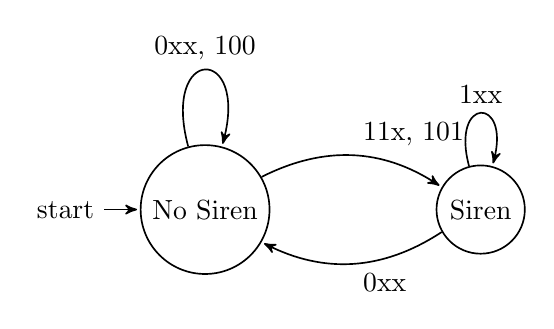
\begin{tikzpicture}[->, >=stealth', shorten >=1pt, auto, node distance=3.5cm, semithick]
    \node[state, initial] (NoSiren) {No Siren};
    \node[state] (Siren) [right of=NoSiren] {Siren};

    \path 
    (NoSiren) edge [loop above] node {0xx, 100} (NoSiren)
              edge [bend left] node {11x, 101} (Siren)
    (Siren)   edge [loop above] node {1xx} (Siren)
              edge [bend left] node {0xx} (NoSiren);
\end{tikzpicture}
\end{document}
